\documentclass{report}

\usepackage[utf8]{inputenc}
\usepackage{polski}

\usepackage{graphicx}
\usepackage{tabularx}

%do edytowania marginesów
\usepackage{changepage}

%Do edytowania list
\usepackage{enumitem}
\setitemize[1]{label={--}}

\title{"Terraria \ppauza poradnik w poczatkowych fazach gry"}
\author{Cezary Kwella}

\begin{document}
\maketitle
\tableofcontents
\listoftables
\chapter*{Wstęp}
\addcontentsline{toc}{chapter}{Wstęp}
\paragraph{} W niniejszym krótkim poradniku chciałbym wyjaśnić podstawowe aspekty gry ,,Terraria'' studia \textbf{Re-Logic}.
\chapter{Początki}
\section{Rozpoczęcie nowej gry}
\subsection{Tryb gry} 
\paragraph{} W menu po włączeniu gry ukaże nam się wybór \textit{trybu gry}. Mamy do wyboru tryb jedno\dywiz i wieloosobowy. Jak sama nazwa wskazuje, od tego zależy, czy będziemy grać sami, czy z innymi \ppauza np. poprzez serwery \textit{steama}.
\subsection{Tworzenie postaci}
\paragraph{} Po wybraniu trybu gry, ukaże nam się okno kreatora postaci. Znajdziemy tutaj następujące opcje:
\begin{itemize}
\item \textbf{wygląd postaci},
\item \textbf{nazwa},
\item \textbf{poziom trudności postaci} \ppauza różnice przedstawiono na  \textbf{tabeli \ref{tab:difficulty}}.
	\begin{table}
	\centering
	\begin{adjustwidth}{-2.4cm}{}
	\begin{tabular}{|p{0.25\linewidth}|p{0.25\linewidth}|p{0.25\linewidth}|p{0.25\linewidth}|}
	\hline
	\textbf{podróż} & \textbf{klasyczny} & \textbf{średni} & \textbf{hardcore} \\
	\hline
	\begin{itemize}
	\item Postać rozpoczyna grę z dodatkowym wyposażeniem,
	\item głównie do testowania,
	\item możliwość cheatowania. 
	\end{itemize} &
	\begin{itemize}
	\item Po śmierci postacie upuszczają tylko (albo i aż) zdobyte pieniądze, 
	\item \textbf{polecany} podczas pierwszej rozgrywki. 
	\end{itemize} & 
	\begin{itemize}
	\item Oprócz pieniędzy po śmierci upuszczane są wszystkie posiadane w ekwipunku przedmioty.
	\end{itemize} & 
	\begin{itemize}
	\item Po śmierci na tym poziomie nie można się odrodzić,
	\item \textbf{wyzwanie} dla bardzo zaawansowanych graczy.
	\end{itemize} \\
	\hline
	\end{tabular}
	\end{adjustwidth}
	\caption{Porownanie trybów trudności gry}
	\label{tab:difficulty}
	\end{table}
\end{itemize}
\subsection{Tworzenie świata}
\paragraph{} Po stworzeniu postaci otworzy nam się nowe okno - kreator świata. 
\begin{figure}
	\centering
	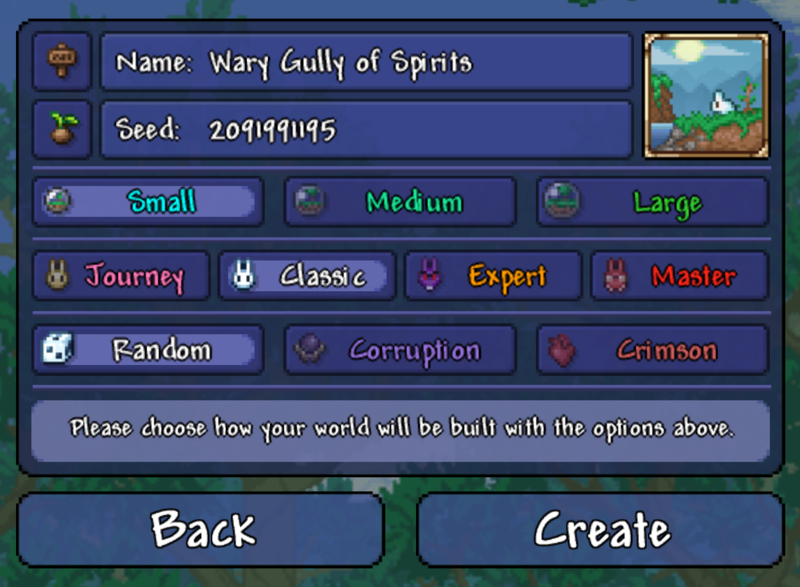
\includegraphics[scale=0.4]{createWorld}
	\caption{Przykładowe menu tworzenia świata w języku angielskim }
	\label{rys:world}
\end{figure}
Na \textbf{rysunku \ref{rys:world}} widać opcje, które możemy ustawić. Są to: 
\begin{itemize}
	\item nazwa,
	\item ziarno generatora,
	\item rozmiar świata,
	\item poziom trudności świata,
	\item rodzaj złego biomu (polecany \textbf{losowy}).
\end{itemize}
\paragraph{} Po wybraniu wszystkich opcji, jeśli jesteśmy gotowi na przygodę wybieramy \textit{Stwórz} oraz rozpoczynamy grę!
\chapter{Pierwsze dni na świecie}
\section{Poruszanie i narzędzia}
\paragraph{} Do poruszania, jak w większości gier będziemy korzystać z \textbf{WASD i spacji}. Aby użyć narzędzia musimy je wybrać korzystając ze \textbf{scrolla} na myszce, a następnie wcisnąć \textbf{lewy przycisk myszy}. Przyciskiem aktywacji domyślnie jest \textbf{prawy przycisk myszy}.
\paragraph{}Po włączeniu świata otrzymaliśmy podstawowe narzędzia, które używamy do różnych rzeczy. I tak kilof pozwala nam niszczyć bloki, siekiera rąbać drzewa, a miecz walczyć z atakującymi nas zewsząd potworkami. Dodatkowo możemy stworzyć młot do niszczenia bloków tła oraz inne rodzaje bronii w późniejszych fazach gry.
\section{Za co warto się zabrać?}
\paragraph{} Łatwo się domyśleć, że na początku najważniejszym będzie zebranie podstawowych surowców, którymi gra nas chce obdarzyć. Warto ściąć trochę drewna oraz znaleźć miejsce na naszą (tymczasową?) bazę. Wybudowanie domu jest istotne w późniejszych facach gry, bo pozwala na osiedlanie się handlarzy, z którymi będziemy mogli handlować za pieniądze zdobyte z potworów, oraz innych NPC.
\paragraph{} Budowa domku nie powinna być niczym skomplikowanym. Gdy mamy zaznaczony nasz materiał wyboru (polecam na początek drewno) wystarczy że wciśniemy (domyślnie) prawy przycisk myszy. \textbf{Uwaga!} Ważne, aby nie stać zbyt daleko od miejsca, w którym chcemy postawić blok. Gdy podstawowy szkielet domu już mamy, możemy zająć się \textbf{craftingiem}.
\begin{figure}
	\centering
	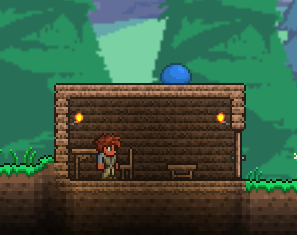
\includegraphics{house}
	\caption{Najbardziej podstawowy domek}
	\label{rys:house}
\end{figure}
\paragraph{} Wciskając klawisz \textbf{Esc} mamy dostęp do poszerzonego ekwipunku i menu. Po lewej stronie ukażą nam się rzeczy, do których scraftowania mamy wystarczająco surowców. Wybierzmy z listy \textbf{Stół warsztatowy}. Po postawieniu, gdy będziemy stali wystarczająco blisko, poszerzy on naszą listę rzeczy, które możemy scraftować. W ten sposób możemy stworzyć drzwi oraz \ppauza jeśli walczyliśmy trochę ze szlamami \ppauza pochodnie.
\paragraph{} Gdy mamy już naszą prowizoryczną kryjówkę (zob. Rysunek \ref{rys:house}) (z drzwiami, stołem, krzesłem, ścianami i pochodniami \ppauza rzeczami, których stworzenie umożliwił nam stół warsztatowy), możemy wybrać się w głębiny świata i zacząć "tworzyć" tytułowe \textit{Terrarium}.
\paragraph{} Kopanie pod ziemią może być bardzo relaksujące. Jednak relaks może nam bardzo szybko przerwać znalezienie jaskini pełnej pułapek i złowrogich potworów. Pod ziemią możemy się napotkać na rudy \ppauza warto je wykopać, aby później z nich móc tworzyć lepsze bronie i narzędzia. Oprócz rud, najczęściej w jaskiniach, możemy napotkać skrzynki, które są źródłem wielu artefaktów.
\chapter*{Zakończenie}
\addcontentsline{toc}{chapter}{Zakończenie}
\paragraph{} Ta część poradnika kończy się w tym miejscu \ppauza w kolejnych omówimy bardziej zaawansowane aspekty gry, jak klasy postaci, czy kolejność zabijania bossów.... tak, w tej grze jest ich wielu. Tymczasem dziękuję za uwagę i do następnego razu!
\end{document}